\chapter[Title of the chapter 5 displayed \\ in the table of contents]
    {Title of the chapter 5 displayed in the page
        \chaptermark{Ch. 5 title in the header}
    }
    \chaptermark{Ch. 5 title in the header}
\label{ch:labelchapter5}

\updatemylof % to be used with "list of figure divider per chapter" (see PREAMBLE)
\updatemylot % to be used with "list of table divider per chapter" (see PREAMBLE)

\regularsection
\headerregularsection

Author 1\textsuperscript{1,\textcolor{sophia}{$\ast$}}, Author 2\textsuperscript{1,2,\textcolor{sophia}{$\ast$}}, Author 3\textsuperscript{3}, Author 4\textsuperscript{1}, Author 5\textsuperscript{1}, Author 6\textsuperscript{1}, Author 7\textsuperscript{2,4,\#} and Author 8\textsuperscript{1,\#} \hfill  \newline

\let\thefootnote\relax\footnotetext{\textsuperscript{1}Department X, University 1, City A, Country B. 
\textsuperscript{2}Department Y, University 2, City C, Country D. 
\textsuperscript{3}Institute E, City F, Country G. 
\textsuperscript{4}Research Center H, University I, City J, Country K. 
\textsuperscript{\#}e-mail: \href{mailto:author7@university2.ac.countryD}{author7@university2.ac.countryD} and \href{mailto:author8@universityI.countryK}{author8@universityI.countryK}}

\noindent First published in: \textit{Scientific Reports} \textbf{10}, 853 (2020). \hfill \break
DOI: \href{https://doi.org/10.1038/s41598-019-55424-z}{10.1038/s41598-019-55424-z} 

\begin{wrapfigure}[3]{l}{0.2\textwidth}
    
\includegraphics[width=0.2\textwidth]{figures/by.png}
\end{wrapfigure} 

\noindent \textcolor{white}{test} \newline \textbf{Open Access} This article is licensed under a Creative Commons Attribution 4.0 International License. It means that unrestricted use, sharing, adaptation, distribution, and reproduction in any medium or format are allowed, as long as the original author(s) and the source are appropriately credited, a link to the Creative Commons license is provided, and any changes made are indicated. To view a copy of this license, please visit \href{http://creativecommons.org/licenses/by/4.0/}{http://creativecommons.org/licenses/by/4.0/}. \newline

\noindent \copyright \ Liudi Mulyo \textit{et al}, 2020. \newline

\noindent \textbf{Contributions} \newline
\noindent \lipsum[2]

%%%%%%%%%%%%%%%%%%%%%%%%%%%%%%%%%%%%%%%%%%%%%%%%%%%%%%%%%%%%%%%%%%%%%%%%%%%%%%%%%%%%%%%%%%%%%%%%%%%%%%%%%%%%%%%%%%%%%%%%%%%

\tcbset{enhanced,colback=abstractback,colframe=sophia,fonttitle=\bfseries}
\begin{tcolorbox}[left=3.35cm,grow to left by=3.5cm,right=3.33cm,grow to right by=3.5cm,title={\normalfont \color{White} \small \fontfamily{bch} \selectfont \scshape Abstract}]
% https://tex.stackexchange.com/questions/232878/inserting-pictures-in-tcolorbox
% https://tex.stackexchange.com/questions/169794/outer-margin-of-tcolorbox/169877
% https://tex.stackexchange.com/questions/11484/how-to-draw-a-frame-box-around-an-arbitrary-large-piece-of-text-figures-whatever
\begin{minipage}[t]{\linewidth}
\vspace*{-29pt}
\phantomsection % to fix wrong hyperref to "Abstract" 
\section*{} % for linking from TOC (only one way)
\addcontentsline{toc}{section}{Abstract}
\begin{sloppypar}
\lipsum[1]
\end{sloppypar}

\end{minipage}

\vspace*{3.5pt}
\end{tcolorbox}

%%%%%%%%%%%%%%%%%%%%%%%%%%%%%%%%%%%%%%%%%%%%%%%%%%%%%%%%%%%%%%%%%%%%%%%%%%%%%%%%%%%%%%%%%%%%%%%%%%%%%%%%%%%%%%%%%%%%%%%%%%%

\begin{sloppypar} % to suppress overfull box

As in \Autoref{ch:labelchapter4}. Lorem \index{Lorem} ipsum dolor sit amet, consectetuer adipiscing elit \cite{LIUDIMULYO201767}. Ut purus \index{purus} elit,vestibulum ut, placerat ac, adipiscing vitae, felis \citenum{LIUDIMULYO201767}. Curabitur dictum \index{dictum} gravidamauris. Nam arcu libero, nonummy eget, consectetuer id, vulputate a, magna. Donec vehicula augue eu neque \cite{liudimulyo_2018}. Pellentesque habitant morbi tristique senectuset netus et malesuada fames ac turpis egestas \index{egestas}\citenum{liudimulyo_2018}. Mauris ut leo. Cras viverra metusrhoncus sem \cite{2019liudimulyo}. Nulla et lectus vestibulum urna fringilla ultrices. Phasellus eutellus sit amet tortor gravida placerat \citenum{2019liudimulyo}. Integer sapien est, iaculis in, pretium quis,viverra ac, nunc. Praesent eget sem vel leo ultrices bibendum \cite{liudimulyo2020853}. Aenean faucibus. Morbi dolor nulla, malesuada eu, pulvinar at (\ref{fig:figures/paper-iv/fig-5}), mollis ac, nulla. Curabitur auctorsemper nulla \citenum{liudimulyo2020853}. Donec varius orci eget risus. Duis nibh mi, congue eu, accumsaneleifend, sagittis quis, diam. Duis eget orci sit amet orci dignissim rutrum \cite{LIUDIMULYO201767,liudimulyo_2018,2019liudimulyo,liudimulyo2020853,liudimulyo_unpublished1,liudimulyo_unpublished2}. For more information, see \hyperref[appendix:B]{Appendix B}, specifically in \ref{tab:appendixB}.

\end{sloppypar}

\begin{figure} % \begin{figure} will let LaTeX decide the best figure placement for you ; \begin{figure}[H] for forcing the figure placement here ; in the bottom, \begin{figure}[!b] ; top of the page, \begin{figure}[!t]
    \centering
    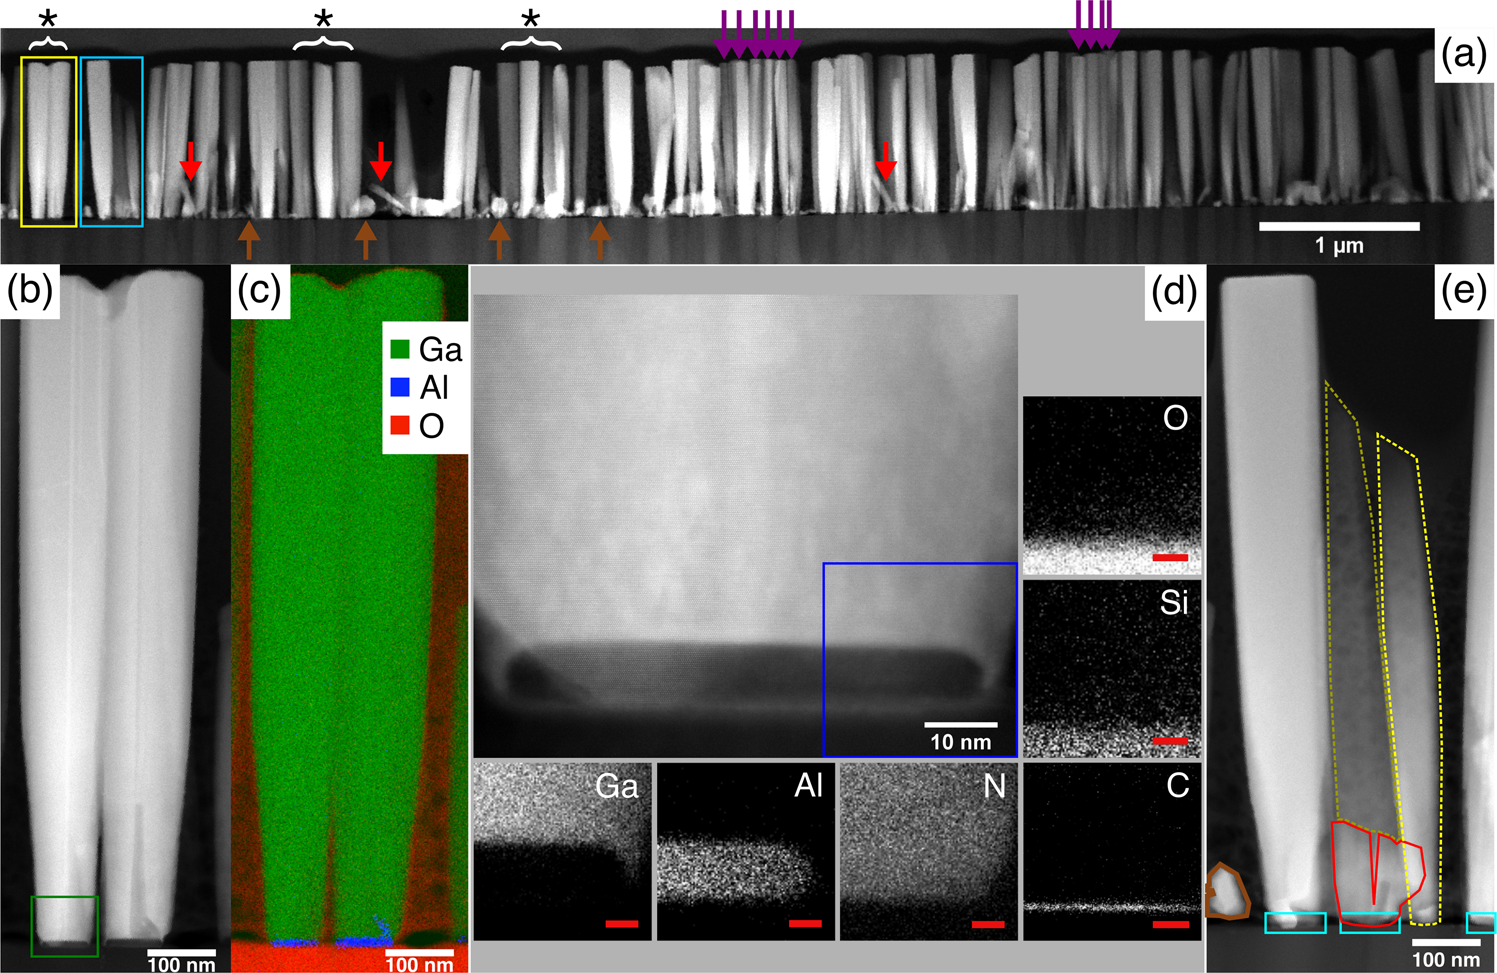
\includegraphics[width=\textwidth]{figures/paper-iv/fig-5.png}
    \caption[TEM image of GaN nanocolumn sample synthesized with\newline nominally the same growth conditions as sample G1]{TEM image of GaN nanocolumn sample synthesized with nominally the same growth conditions as sample G1. (\textbf{a}) Overview cross-sectional HAADF STEM image, showing vertical GaN nanocolumns (star-marked and purple arrows), inclined GaN nanocolumns (red arrows) and GaN crystallites (brown arrows). (\textbf{b}) HAADF STEM image of two GaN nanocolumns within yellow frame in \textbf{a}. (\textbf{c}) Combined color map of the Ga (green), Al (blue) and O (red) elemental distributions (EDS/EELS) on the corresponding region in \textbf{b}. (\textbf{d}) Magnified image of the lower part of the GaN nanocolumn near the interface of the left GaN nanocolumn in \textbf{b} (green frame), with the elemental mapping near the interfaces between the GaN nanocolumn, AlN island, graphene and silica glass (blue frame) by EDS (Ga, Al, Si) and EELS (N, O, C). The red scale bars are 5 nm. (\textbf{e}) HAADF STEM image of the GaN nanocolumns that is light-blue framed in \textbf{a}. The inclined GaN nanocolumn (yellow-dashed line) is possibly directly nucleated on graphene (indicated by the absence of any AlN layer [cyan frames] at the base). There are two broken GaN nanocolumns (red framed area) sharing the same AlN island and another inclined GaN nanocolumn (dark-yellow dashed line) in the background. An irregular GaN crystallite (brown outline) likely grown directly on graphene is also observed (adapted with permission from ref. \citenum{liudimulyo2020853} \copyright \ Liudi Mulyo \textit{et al}, 2020.}
    \label{fig:figures/paper-iv/fig-5}
\end{figure}

\section{Section 1 in chapter 5}
\lipsum[2-4]

\subsection{Subsection 5.1 of section 1 in chapter 5}
\lipsum[5-7]

\subsection{Subsection 5.2 of section 1 in chapter 5}
\lipsum[8-11]

\clearpage\phantomsection % to fix wrong hyperref to this section
\section[Long section title displayed in the table of content]{Short section title in the chapter}
\sectionmark{Even shorter title on the header}
\lipsum[11-18]
See \ref{tab:ch5}

\begin{table}[!h]
\centering
\caption{Micro-Raman peak positions, intensities and ratios}
\label{tab:ch5}
{\fontsize{7}{6}\selectfont
{\renewcommand{\arraystretch}{2}
\begin{tabular}{cccccccc}
\toprule
\multirow{3}{*}{\textbf{Sample}} & 
\multirow{3}{*}{\textbf{\begin{tabular}[c]{@{}c@{}}Median\\ D/G ratio\end{tabular}}} & 
\multicolumn{2}{c}{\textbf{Median G}} & 
\multicolumn{3}{c}{\textbf{Median 2D}} & 
\multirow{3}{*}{\textbf{\begin{tabular}[c]{@{}c@{}}Median \\ 2D/G ratio\end{tabular}}} \\
\cmidrule(l){3-4} \cmidrule(l){3-4} \cmidrule(l){3-4} \cmidrule(l){5-7} \cmidrule(l){5-7} \cmidrule(l){5-7} % repeated three times to increase the line thickness
  &  & \textbf{\begin{tabular}[c]{@{}c@{}}Position \\ {[} cm\textsuperscript{-1} {]}\end{tabular}} & \textbf{\begin{tabular}[c]{@{}c@{}}Intensity \\ {[} cps {]}\end{tabular}} & \textbf{\begin{tabular}[c]{@{}c@{}}Position \\ {[} cm\textsuperscript{-1} {]}\end{tabular}} & \textbf{\begin{tabular}[c]{@{}c@{}}Intensity \\ {[} cps {]}\end{tabular}} & \textbf{\begin{tabular}[c]{@{}c@{}}FWHM \\ {[} cm\textsuperscript{-1} {]}\end{tabular}} &  \\
\midrule
\begin{tabular}[c]{@{}c@{}}DLG before\\ MBE growth\end{tabular} & 1 & 2 & 3 & 4 & 5 & 6 & 7 \\
\rowcolor{Gray} \begin{tabular}[c]{@{}c@{}}DLG after\\ MBE growth\end{tabular} & 1 & 2 & 3 & 4 & 5 & 6 & 7 \\
\bottomrule
\end{tabular}
}
}
\end{table}

\subsection{Subsection 5.2 of section 2 in chapter 5}
\lipsum[13-14]

%=======================================================================
%%% References 

% \clearpage
\phantomsection
\specialsection % put an indent, see preamble
\headerspecialsection

{\hypersetup{urlcolor=ntnu,linkcolor=sophia} % set clickable URL title color to black, not ntnu like in the main document

\bibliographystyle{unsrtnat-mod}  % NATBIB ref style
\bibliography{references}
}